\documentclass{extarticle}

\usepackage{graphicx}
\usepackage[utf8]{inputenc}
\usepackage[russianb]{babel}


\begin{document}

\title{СИМУЛЯЦИЯ MITM атаки в PEAP посредством HOSTAP}

\date{Декабрь 27, 2016}

\author{Сергея Синяк. Виктор Синяк}

\begin{abstract}
  Исходная цель заключалась в следующием:
  Так если я тот самый пльзователь, который опускает
  проверку сертификата,
  и сеть использует ту самую конфигурацию ---
  PEAPv0,v1  с MSCHAPv2.
  То почему бы не поиспользовать других не подзревающих
  об этом пользователей,
  написан реальный эксплоит.
\end{abstract}

\maketitle

\section{Введение}

Я бы хотел продемонстрировать анализ PEAP,
с последующей реализацией MITM эксплоита.
Суть заключается в симуляции атаки.
В качестве отправной точки была принята публикация
\cite{tap2002},
датирования 2002, полученая и опубликованая в 2013ю
Там мы наблюдаем исследование туннелированных протоколов
аутентификации.
Подавляющее большинство унаследованных, а следовательно
широко распостраненных протоколов
требуют обновления, дабы соотвествовать последним
стандартам безопасности.
При этом сильно важно сохранить унаследованный код
и инфаструктуру.
Если протокол подвержен проблемам слабого пароля
или не скрывает личность пользователя,
то он может быть протуннелирован некоторым внешним протоколом.
В этом случае, сервер сетевого доступа
аутентифицируется для клиента внешним протоколом,
а затем клиент аутентифицируется для сервера внутренним
(предпологаемо унаследованным).
Как только протокол завершен, обе стороны завершают коммуникацию
генерацией токенов,
в случае успешной аутентификации.
Если мы говорим о зашифрованном сетевом доступе,
то результирующие токены есть сессионные ключи,
которые определяют шифрование дальнейших сообщений
передача которых произойдет посредством
канал связи, который и был аутентифицирован.

\section{Криптобиндинг}
Внутренний протокол должен бы криптографическ связан
с внешним.
Работа \cite{tap2002} упоминает два пути:
\begin{enumerate}
  \item неявный способ, то есть результирующий ключ $K$ получен
    путём односторонней хэш функции, которая затрагивает как секретные
    данный внешнего протокола $T$,
    там и секретный ключ $S$ из внутреннего протокола.
  \item явная криптографическое связывание, это когда
    особенное значение проверки $V$
    сгенерировано тем же способом из $T$ и $S$,
    и проверено некоторой аутентифицирующей сущностью
    на равенство между сторонами.
\end{enumerate}

Для снижение наложенных правок в унаследованном протоколе,
все эти соображения следует принять в рассмотрение
на уровне внешнего протокола.

Это очень важно добавить криптографическое связывание,
потому что в противном случае внутренний протокол
аутентификации применяется будучи не сведомым о том,
существует ли защищающий туннель или нет.
Такая криптографическая схема является уязвимой к атаке
человек-по-середине.

\section{PEAP с MSCHAPv2}

Давайте рассмотрим PEAP с MSCHAPv2, что часто используется
в Wi-Fi сетях для аутентификации клиентов.
Главная схема имеется название WPA-Enterprise,
и воплошает обычный WPA/WPA2 стандарт зашифрованной беспроводной коммуникации.
Принципиальное различие в аутентификации и выводе сессионных ключей.
В то время как обычный WPA/WPA2 стандарт полагается на одну парольную фразу,
которая известна всем пользователям беспроводной точки,
Промышленная версия разрешает полноценную аутентификацию посредством
EAP конечного автомата.
Это концепт аутентификации общего назначения для разнообразной коллекции
унаследованных, широко распостраненных схем.
На пример, вы можете задействовать Базу пользователей Windows Server'а
настроив сервер сетевого доступа на протокол PEAP с MSCHAPv2
который будет подключаться через RADIUS протокол к серверу и аутентифицировать
пользователя внутри защищенного TLS тунняля через MSCHAPv2 схему.
В начале клиеет, аутентифицирует NAS путём проверки сетевого сертификата,
это происходит в течение протокола TLS Handshake.
Сервер, будучи успешно аутентифицирован и аувторизирован, даёт начало
инициализации обеими сторонами TLS туннедя,
через генерацию общего главенствующего ключа TLS.
TLS схема дозволяет создание общих секретов для обоих сторон,
и является защищенной против атак рода человек-по-середине,
если только пользователь или серевер не пропускают проверку сертификата.
Это стоит того, чтобы отметить, а именно, многие платформы
позволяют тем или иным путём, игнорировать проверку сетевого сертификата сервера,
оставляя пользователей незащищенными.
Практика такого бездумного поведения исходит от использование
самоподписанных сертификатов для аутентификации и работы TLS.
И если соотвествующие уполномоченные не беспокояться о предоставлении
сертификата пользователям
и иногда даже стимулируют опускание проверки,
пользователи, в этом случае, обычно стоят перед выбором
использовать небезопасную сеть,
или отказаться от её ресурсов.
Некоторые замятет, что мы можем применить фиксирование сертификата,
что немного более безопасно, чем не проверять его вовсе.
Да, мы действительно можем это.

\section{Tools analysis}

The original goal was the following:
So if I am the very user who skips certificate verification,
and the network uses the very exact configuration - PEAP with MSCHAPv2.
Then why not to abuse other unsuspecting users,
by writing a real life exploit.

Among the available tools,
hostap project \cite{hostap-w1fi} looked as very prominent.
Because it is the implementation of both client and server side
of wireless network encryption schemes.
The codebase is up-to-date, widely sprea,
actually all Android phones, and for sure almost every linux machine
uses its wpa\_supplicant, that is a client application for authentication
and session key derivation in Wi-Fi networks.
The hostapd application represents a server-side counterpart
to wpa\_supplicant.
The application architecture is modular, and contains implemented EAP state machine
for both peer and server.
Even more, there is a working example, that simulates communication
of two EAP state machines - peer and server. The configured protocol
is the exact PEAP with MSCHAPv2.

I can't find any serious disadvantages in this direction.
Though few facts should be mentioned.
There is a presentation dated to 2008,
from the security conference SHMOOCON 2008 \cite{whfs-peap-shmoocon-2008}.
Two people were talking about server impersontation
to real clients,
but their attack aims to collect
victim's messages during MSCHAPv2 protocol,
then sends authentcation completed successfuly to them.
Those messages allows quick dictionary attack onto the password.
They even presented a patched version of hostapd (hostapd-wpe \cite{hostapd-wpe})
that implements their exploit.
The server gathers special hashes,
that can be cracked by their utility, by name asleap.
Though, it is definetely recalls to our goal,
it is a different attack.
They are cracking weaknesses of password hashing in MSCHAPv2,
and we are going to proxy the whole protocol conversation
and are not interested in its contents.
So you see hostap was already used for similar purposes.
I am not aware of how quickly the password attacking happens,
but I think it takes more time than a simple pass-through of the messages
between a client and a real NAS via MITM node.

\section{MitM attack simulation and its code}

The code \cite{GMI} we present only simulates the attack,
and is not yet a real life exploit.
Let's left the estimation of how far it is away from one
to others.

A straight-forward implementation you may find in \cite{tap2002},
it is as follows:
\begin{enumerate}
  \item MitM waits for a legitimate device to enter an untunneled legtacy remote
    authentication protocol
    and captures the initial messages sent by the legitimate client.
  \item MitM initiates a tunneled authentication protocol with an authentication
    agent.
  \item After the tunnel is set up between MitM and the authentication agent,
    the MitM starts forwarding legitimate client's authentication messages
    through the tunnel.
  \item MitM unwraps the legacy authentication protocol messages received through
    the tunnel from the authentication agent
    and fowards them to the legitimate client.
  \item After the remote authentication ended successfully,
    MitM derives the session keys from the same keys it is using for the tunnel.
\end{enumerate}

The original eap\_example was extended to 4 EAP state machines,
i.e. Bob Peer, Alice Server, Eve Peer and Eve Server.
Here Bob plays the role of a victim,
and Alice is the original server.
Eve Peer and Server state machines represent
a man-in-the-middle,
where it is onvious,
that Bob Peer communicates Eve Server,
and Alice Server authenticates Eve Peer.

In a real life, MitM can intercept by producing a hotspot with the same
"outlook" but with more powerful signal than the original server.
If the network has no encryption,
then the quickest way to perform MitM attack is to enable mobile
internet on your Android phone,
then create a hotspot with a name equal to the access point under attack.
After you need to come close to the victim.
On the internet there is aircrack-ng package,
that allows to send a direct deauthentication packet,
so that client's supplicant is to reinitiate session,
and with a high certainty, your phone will be a chosen one as NAS.

But such a scheme does not work for encrypted network communication,
unless you know the password to impersonate a server,
or any other relevant secret for correct authentication.

In our case, i.e. with WPA-Enterprise hotspot,
configured with PEAP with MSCHAPv2, MitM can be applied,
but mobile internet won't work, as the authentication occurs at the real network
access server, that we can not simulate. We don't know user password.

We can impersonate NAS during TLS Handshake protocol.
Because the only proof of server's identity is the network certificate,
presumably self-signed or provided with a chain toward one of the trusted
Certificate Authorities. But if the client does not verify it,
and such an option is available uniquetuously,
then MitM attack is trivial.
All we need is to participate in TLS Handshake communication.

It is the first phase in PEAP. After that the MSCHAPv2 protocol takes place.
It is tunneled through TLS protocol.

On the figures 1, 2, 3 you may see an original PEAP session, the general
session of MitM attack, and clarified MSCHAPv2 proxying in our implementation.

\begin{figure}
  \centering 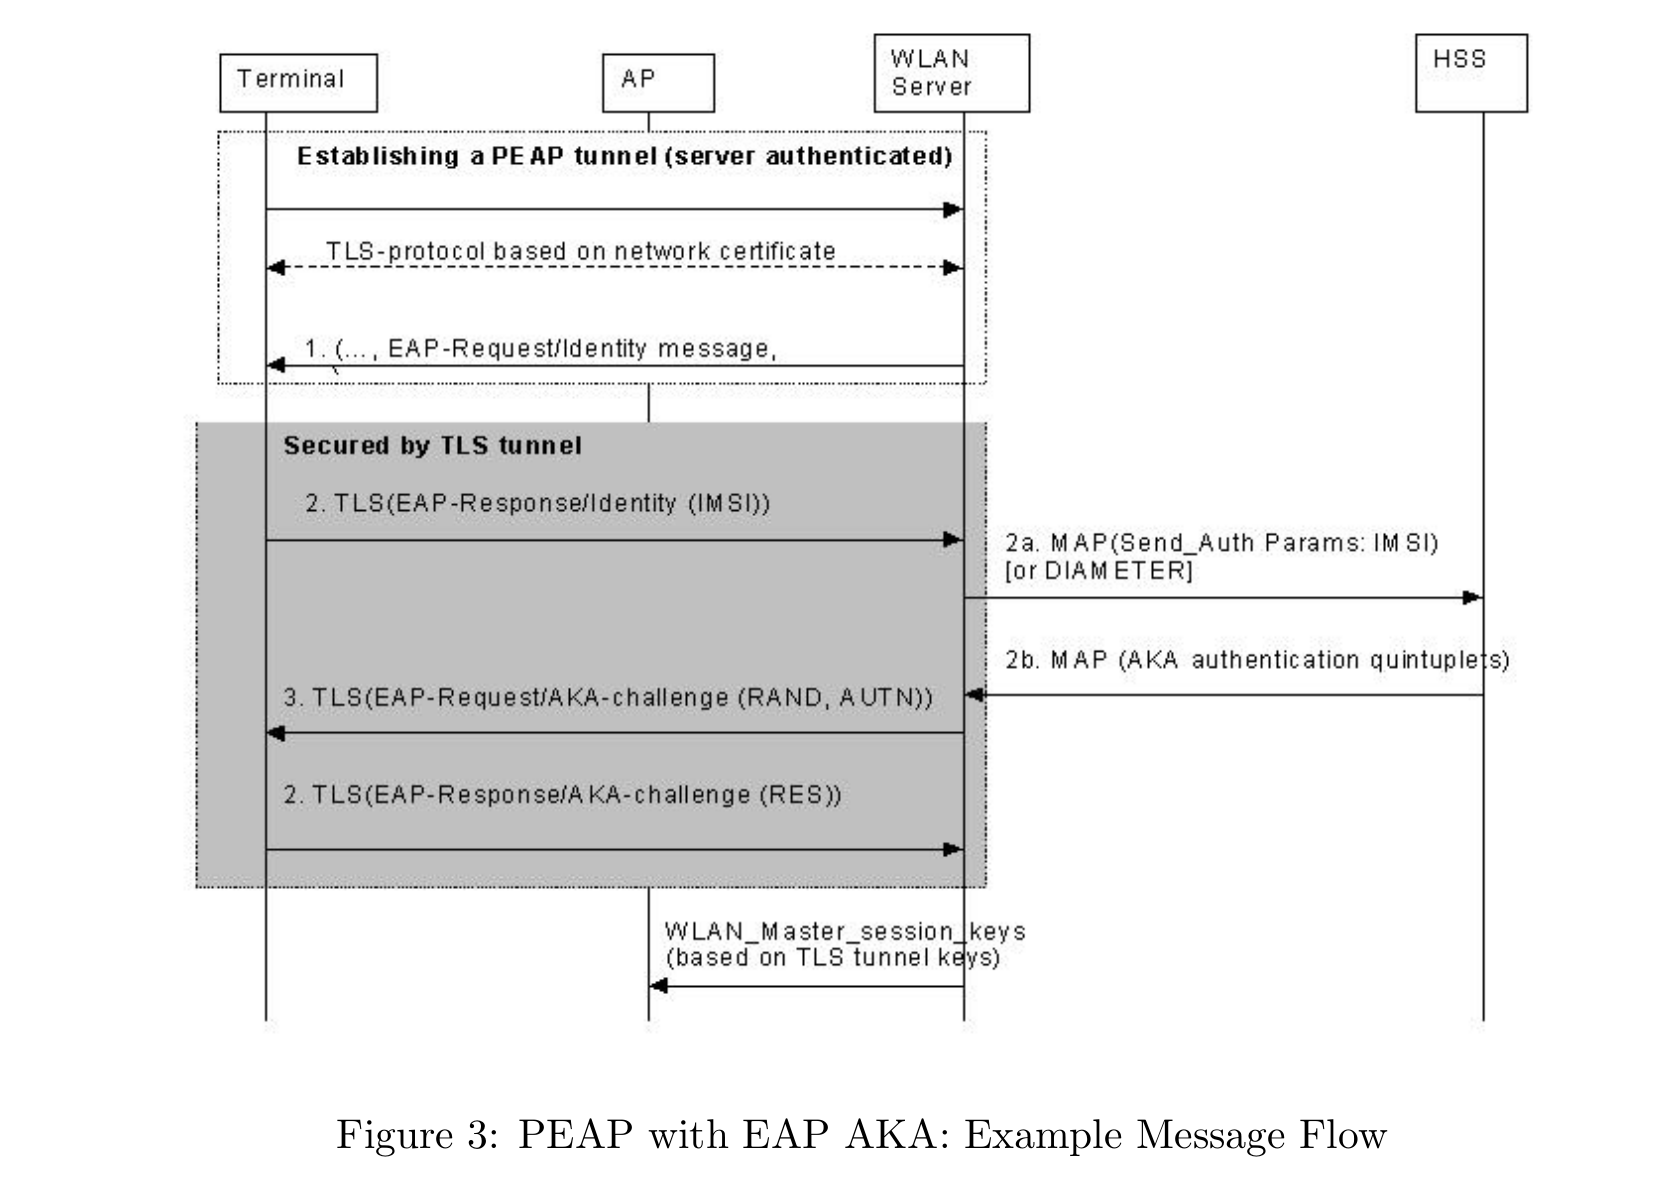
\includegraphics{res/peap-session-fig.png}
  \caption{Обычная сессия PEAP}
\end{figure}

\begin{figure}
  \centering 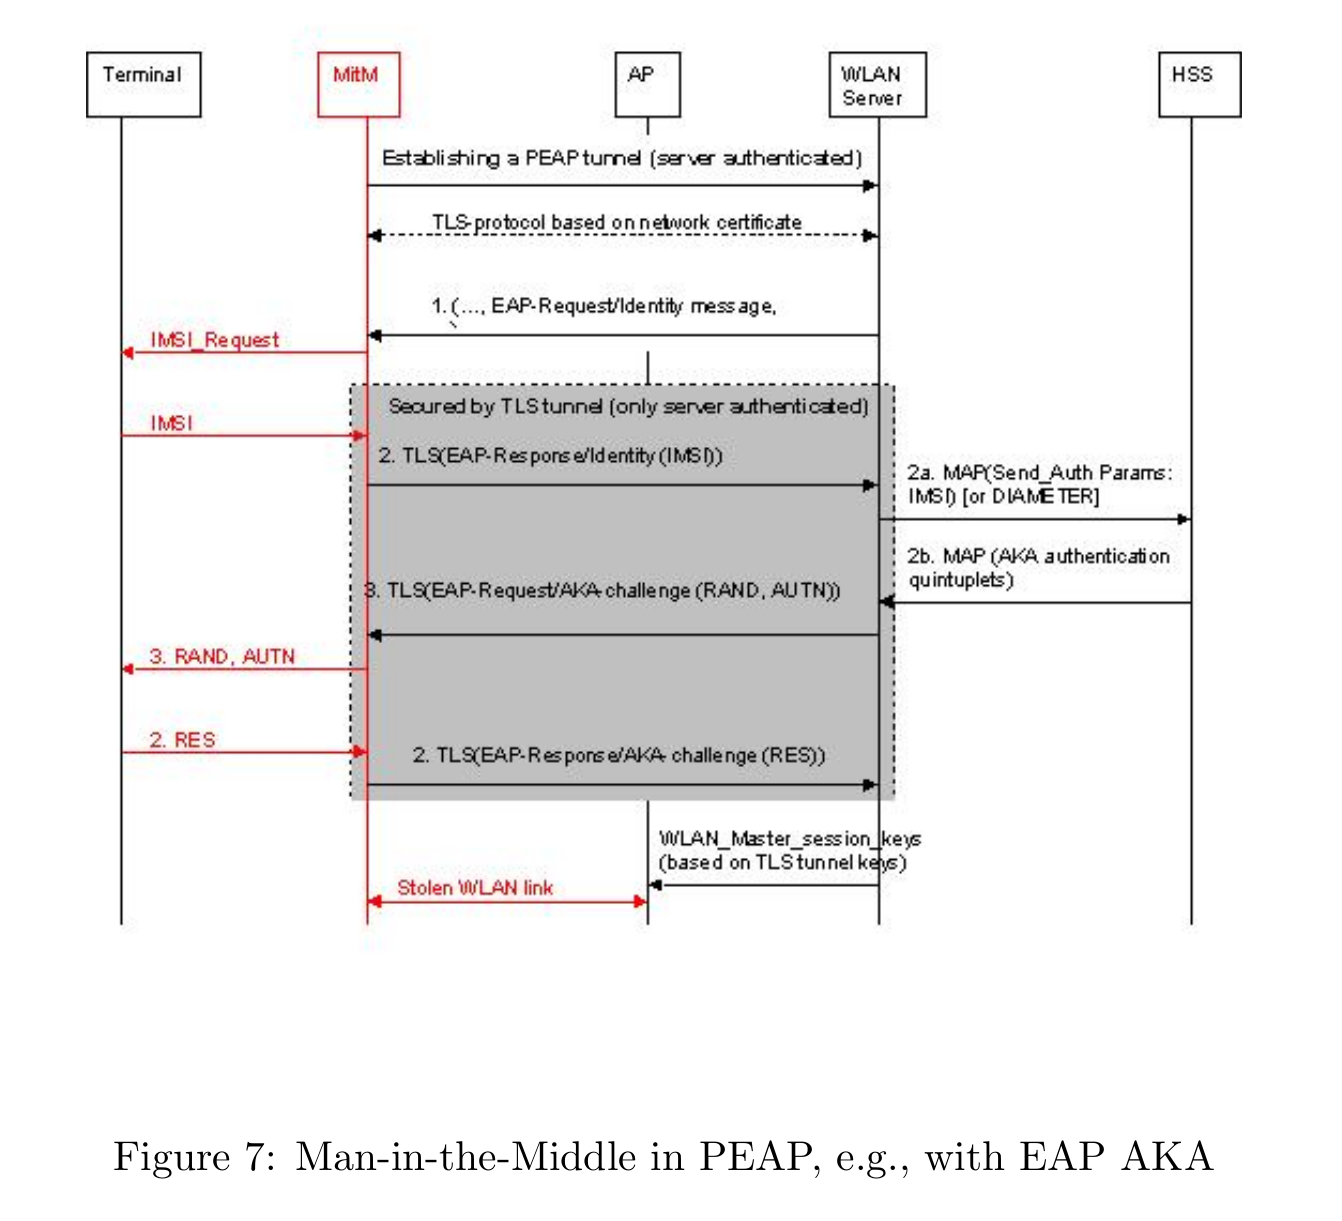
\includegraphics{res/peap-mitm-general.png}
  \caption{Общий вид сессии атаки человек-по-середине в PEAP}
\end{figure}

\begin{figure}
  \centering 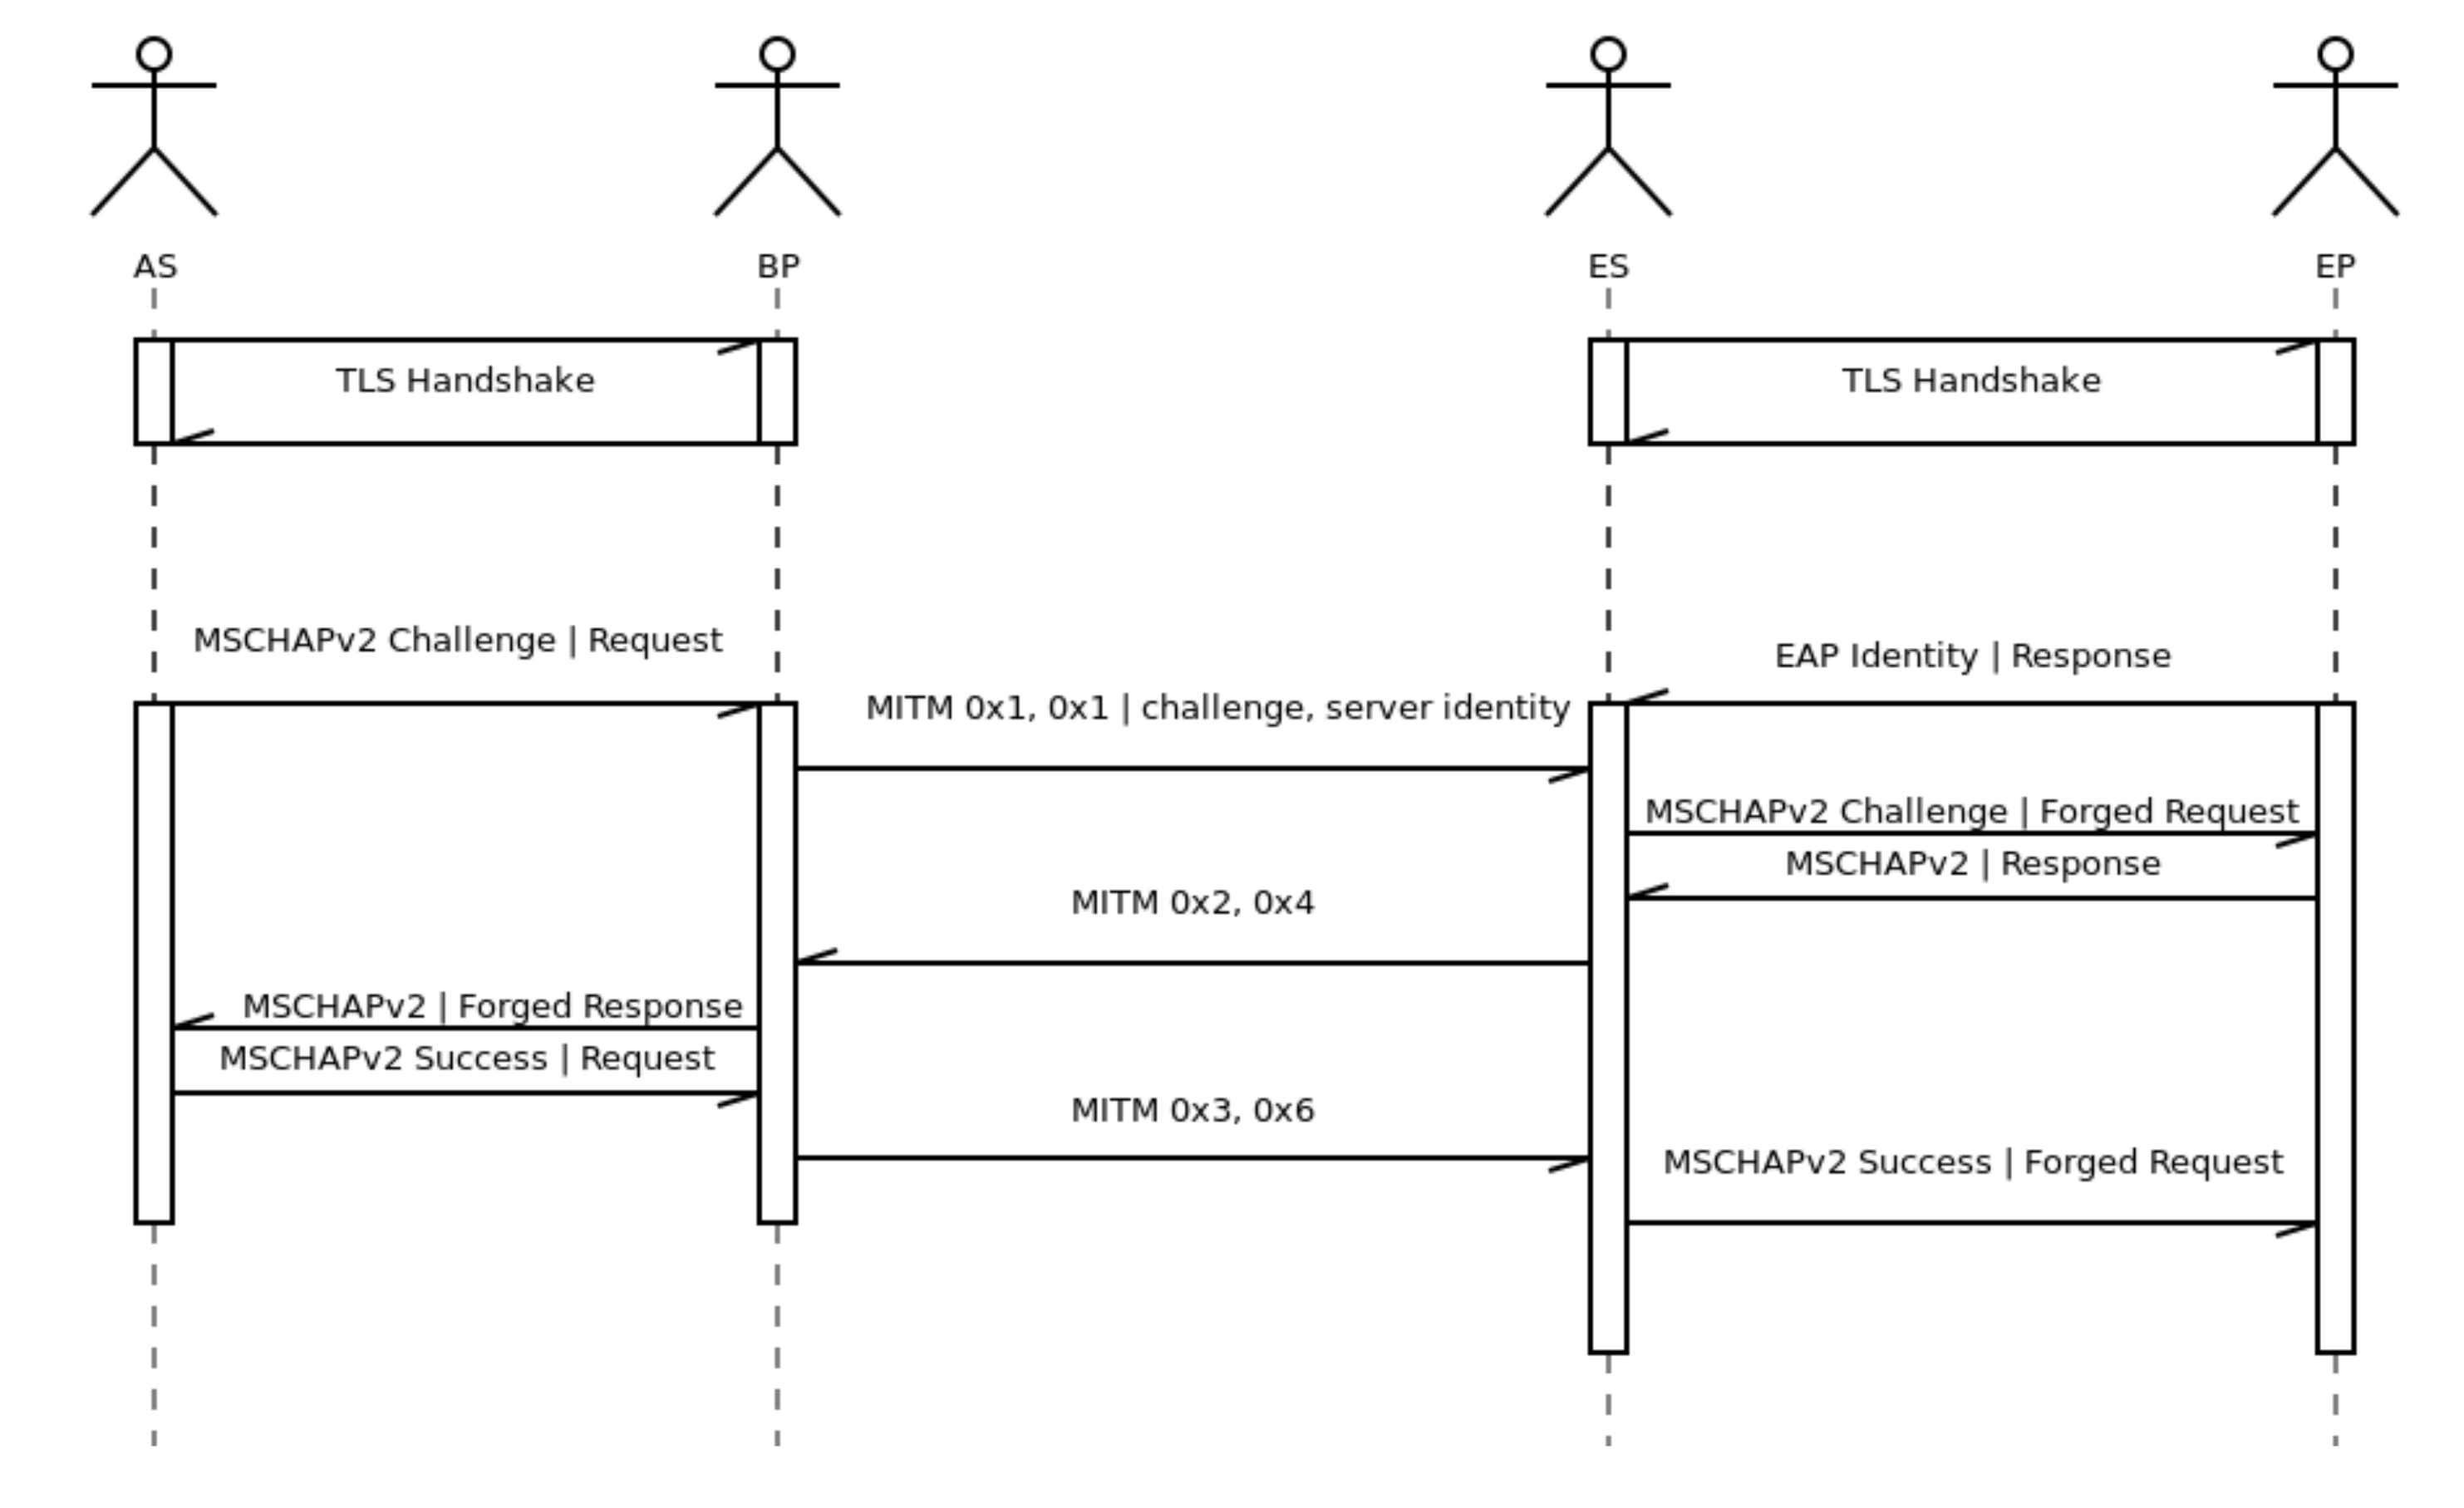
\includegraphics[scale=0.5]{res/clarified-mschapv2-mitm-in-peap.png}
  \caption{Детальная проброска MSCHAPv2}
\end{figure}

\subsection{Codebase analysis}

To acheive the desired behaviour it is important to understand
how the particular implementation operates. Luckily,
the code correspondes wll with RFC 4317, where the architecture of EAP state
machine is defined in details.
There are both EAP Peer and EAP Server state machines.
For the EAP Server the stand-alone authenticator was considered.

First of all we've tested the dfeault behaviour,
it was of great importance to see when the vulnerability exists and when
it does not.
Cryptobindings mentioned in \cite{tap2002} are implemented indeed:
the session key is derived by Pseudo Random Function Plus (PRF+),
it is based on TLS master secret $T$ and phase2 key $S$
derived near the end of inner protocol authentication.
The detailed algorithm is available in \cite{josefsson-draft-10}.
It is worth mentioning that the version 5 \cite{josefsson-draft-05}
of the same draft
states for session key to be derived solely based on TLS master secret $T$.
The search on the internet says that Cisco routers has crypto binding since 2004,
but the functionality is optional.
In hostap, we've discovered that TLS Cryptobinding
(the actuall name of binding protocol)
is always initiated by the server,
and includes not only explicit binding,
but as well generates session key based on $T$ and $S$.
If the crypto binding are disabled,
the behaviour is from \cite{josefsson-draft-05},
i.e. vulnerable to MitM attack,
of course if only the client does not verify the network certificate.

From the code I see that:
\begin{enumerate}
  \item cryptobinding are only present for PEAPv0,
    PEAPv1 implementation does not have this feature,
    and in many aspects resembles PEAPv0.
  \item client can't ask the server to proceed with cryptobinding,
    he can only reject the connection.
    It happens, when client's settings force
    cryptobinding, but the server does not use them, or makes it optional
    in hostap config.
\end{enumerate}

So we disable Bob Peer's verification of server's certificate,
i.e. provide no certificate in config.
Then to disable cryptobinding we force PEAP version on both sides
to be the first. To make some fun,
MitM verifies server's certificate, but forces PEAPv1.
Additionally, Eve Peer and Serer are left without any user password.
Though to make it easier, username is left unchanged
as in original eap\_example code.
Anyway it can be obtained , as the client sends his identity twice,
before TLS Handshake (according to PEAP),
and within TLS tunnel before the inner authentication protocol.
And it is in plain text.

\subsection{Specific notes about hostap implementation}

Now we are going into more details with explanation of hostap implementation.

Originally EAP state machine does not allow pending responses
and requests. But in the MitM attack
Eve Peer and Server are to wait for Bob Peer and Alice Server from time to time.
It appears that such a behaviour was necessary and hostap developers provided
this functionality.
On our side we are using it a lot,
though modification to the PEAP
code was necessary to correct behaviour.
Pending functionality played an important role in interruption of state machine
with its consequent resuming.
Usually TLS has the protection against replay attacks,
and we were not able to replay the PEAP message for Eve's state machines,
when we've obtained necessary data,
to continue with MSCHAPv2 proxying.
But pending allows it by a simple callback,
that keeps decrypted data from the correct message,
and resumes later the method with the same data,
stored at the previous step.
The new packet is ignored if the machine was in pending state.
But it does a favour by triggering all necessary state machine
actions, that perform the resuming. Without that,
the resulting code would be quite cumbersome.

State machine means a graph, were states (vertices) are connected
via directed transitions (arcs), that prescribe the conditions
and the actual direction of state changing.
A machine might perform some actions when it enters a state,
or when it performs transition.
EAP state machines contain actions within states.
In the MitM state machine, we perform actions during state changing.

On figures 4, 5 and 6, 7 are presented EAP Peer, EAP Server and MitM Peer
and Server state machines.



\begin{figure}
  \centering 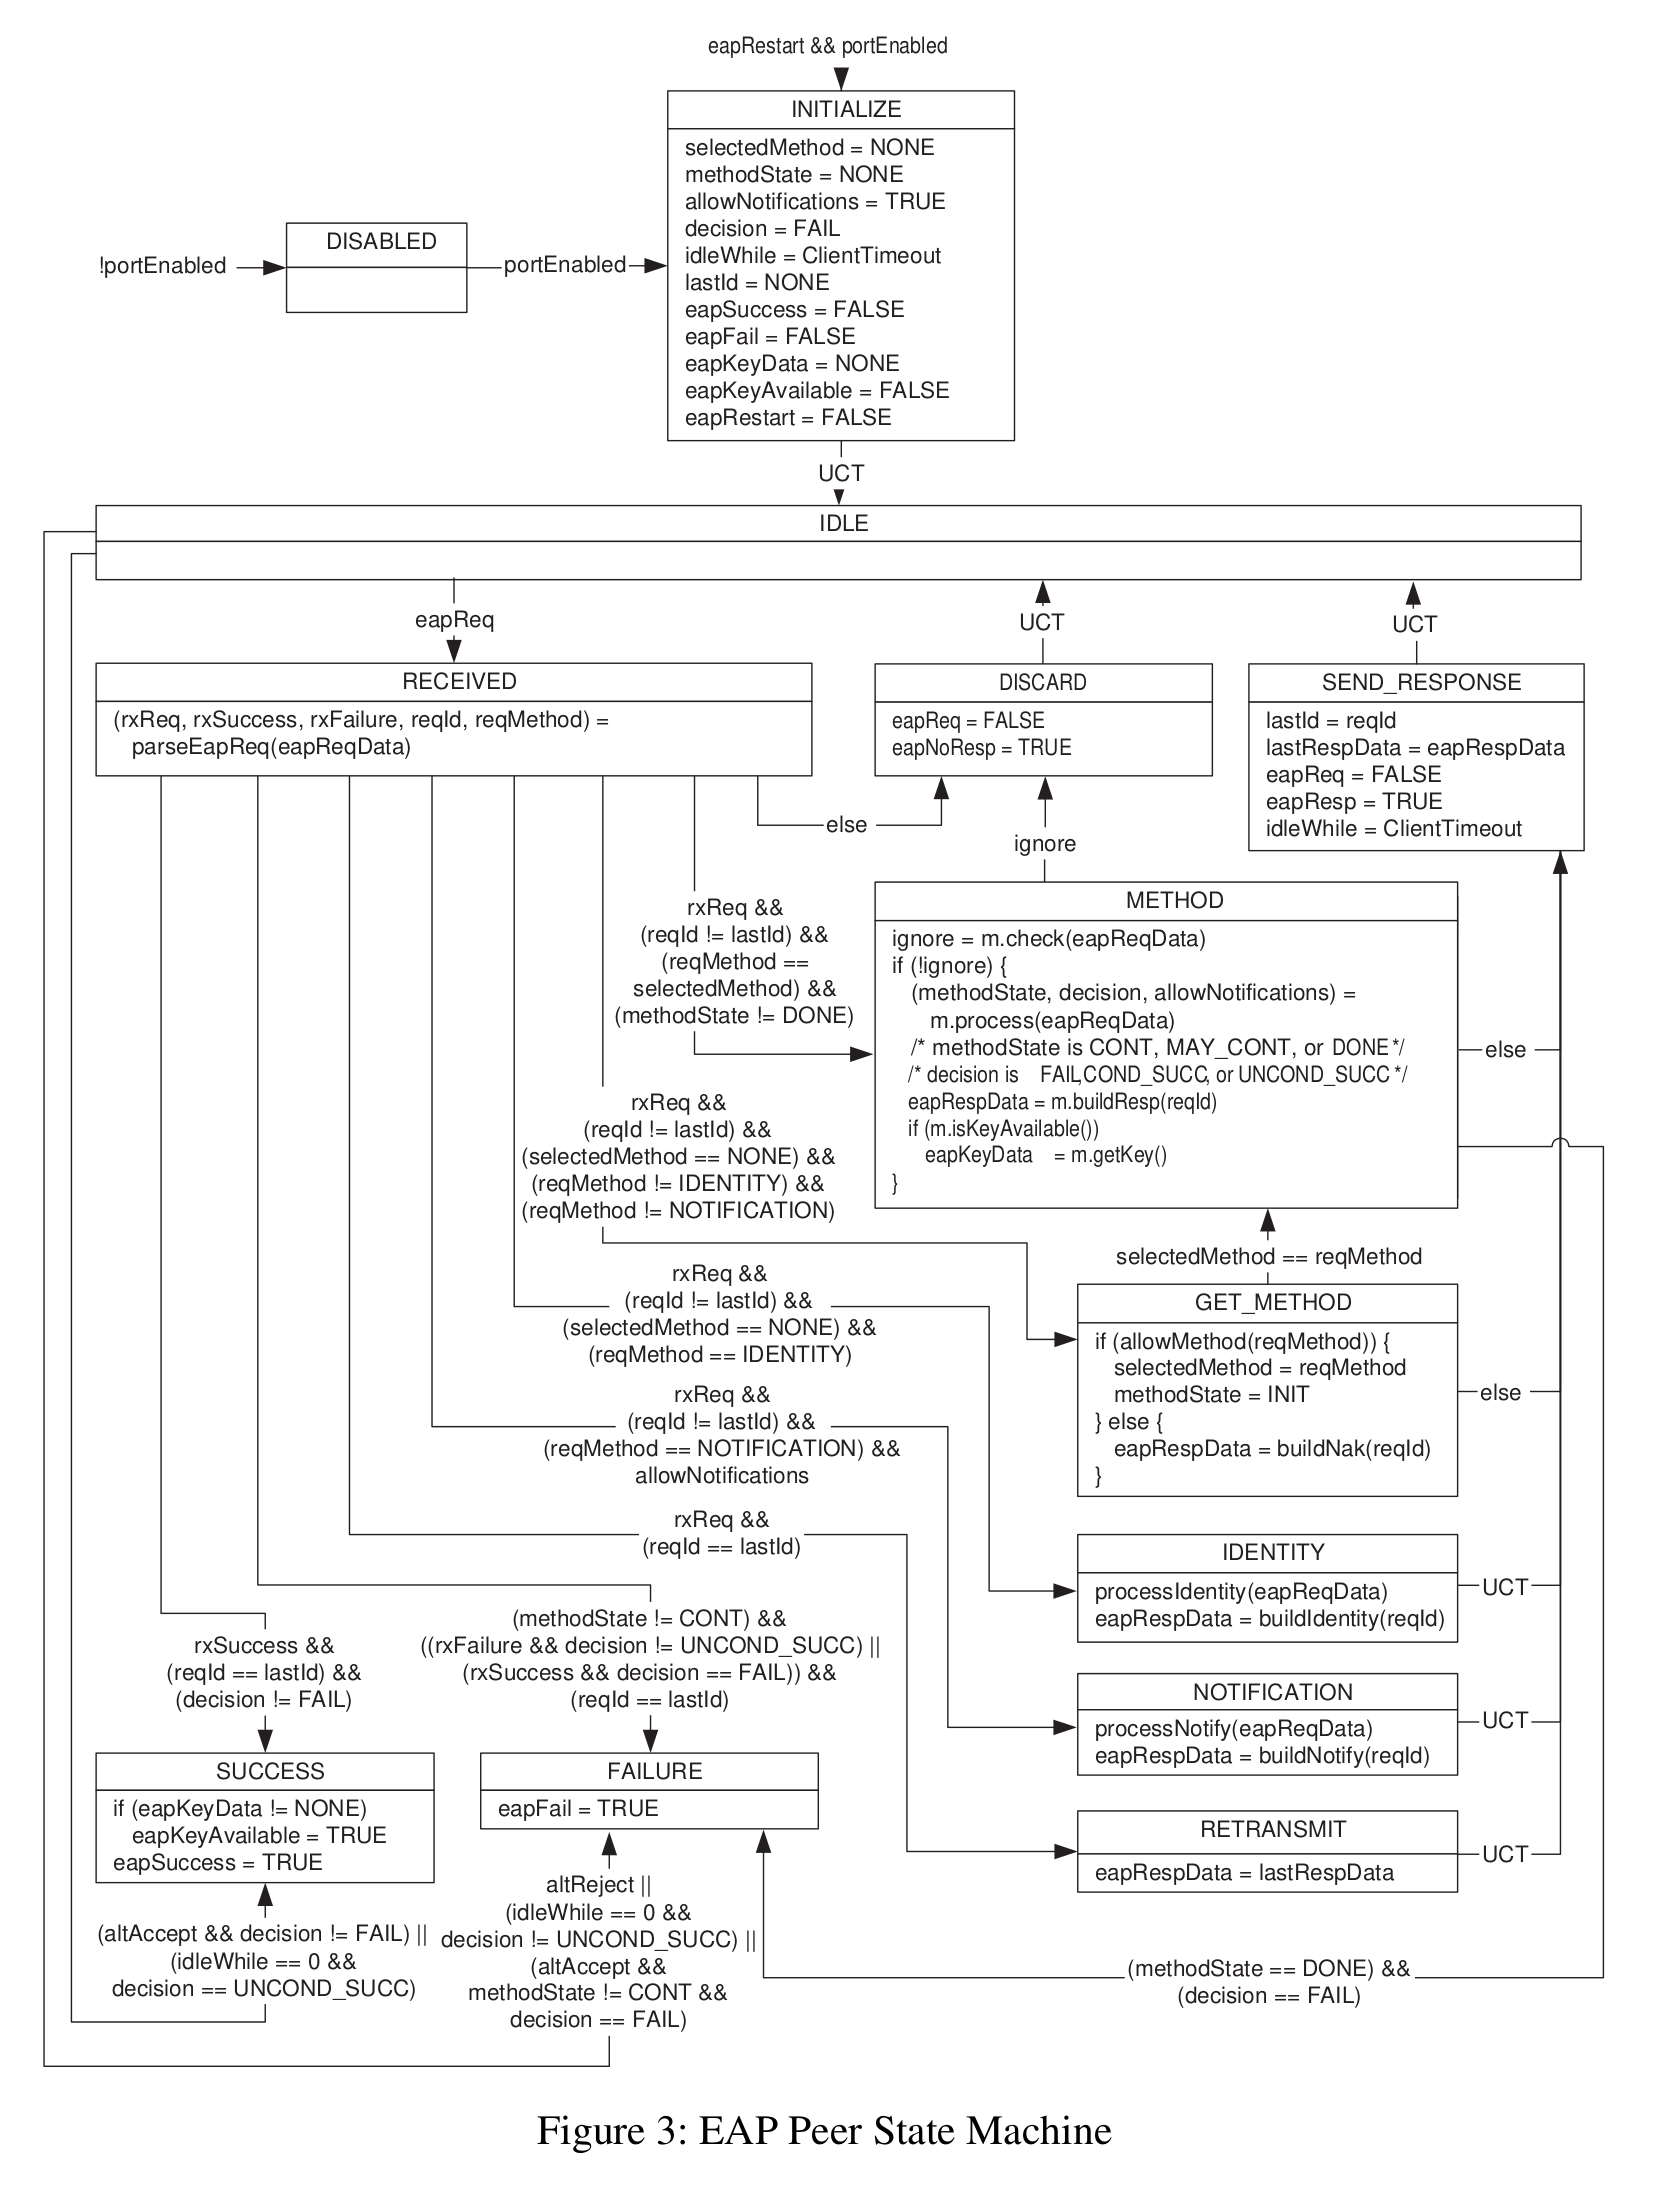
\includegraphics{res/eap-peer-state-machine-rfc4137.png}
  \caption{Автомат EAP Клиента, из RFC4137}
\end{figure}

\begin{figure}
  \centering 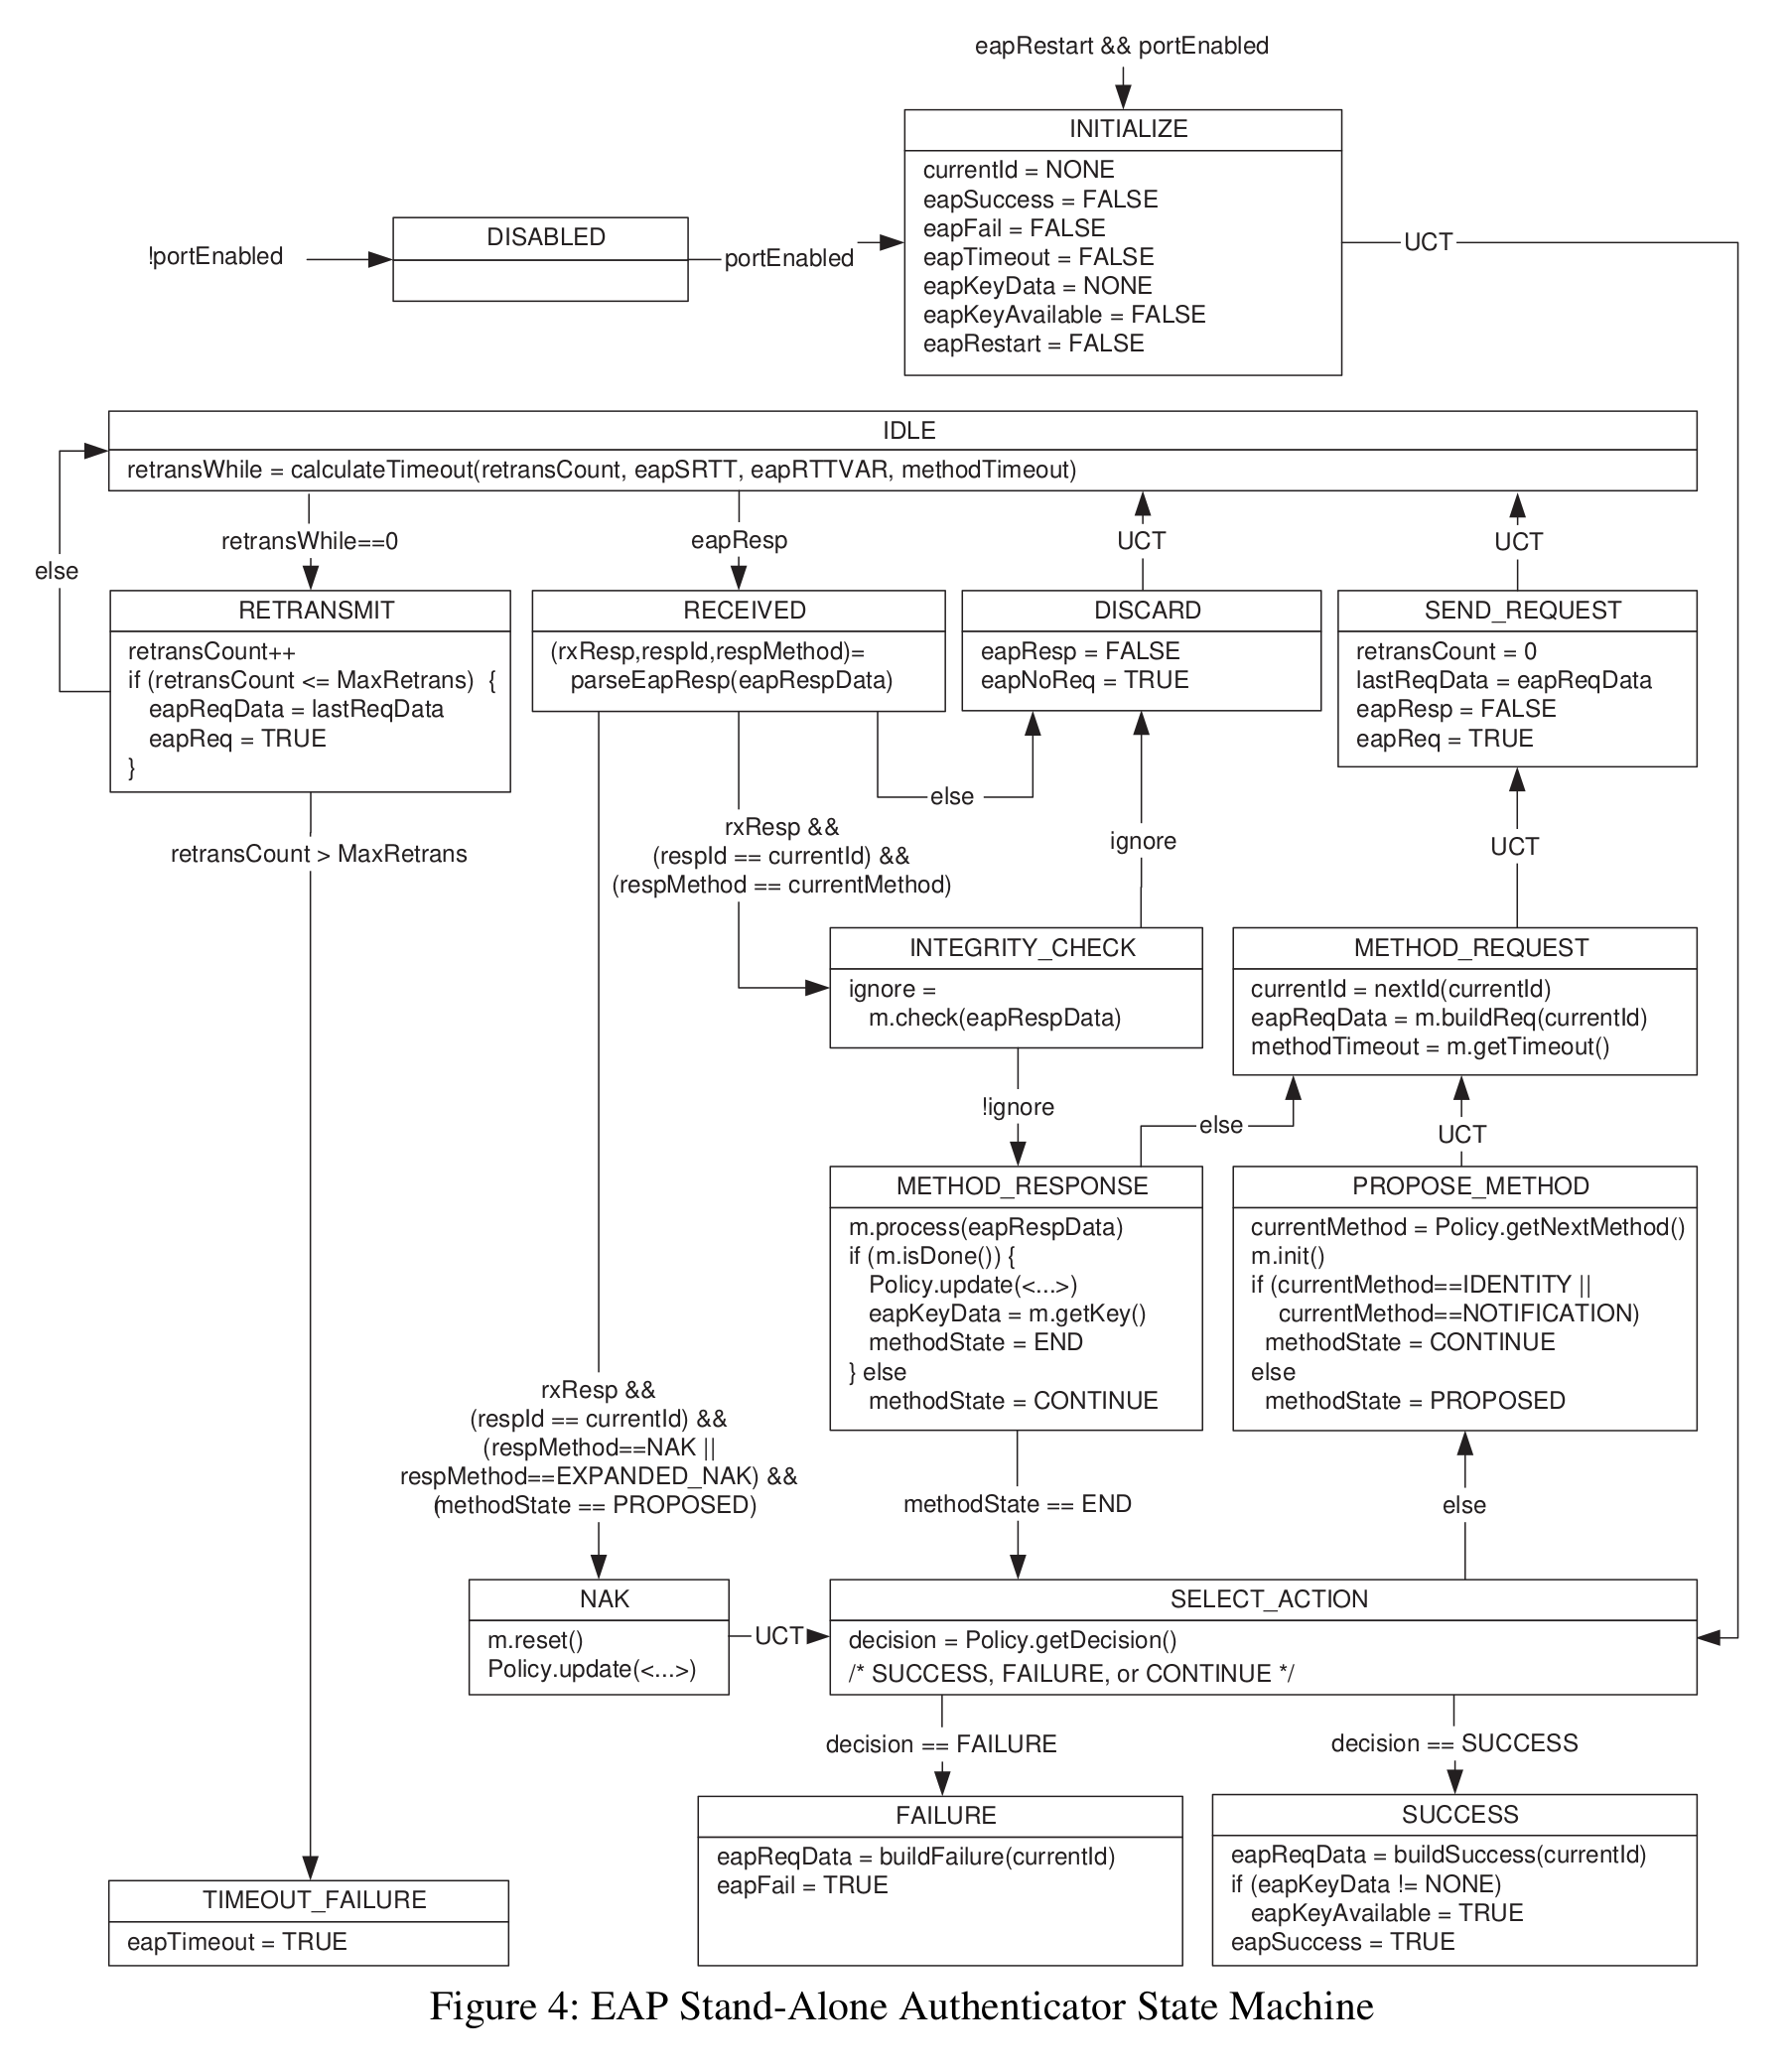
\includegraphics{res/eap-server-state-machine-rfc4137.png}
  \caption{Автомат EAP Сервера, из RFC4137}
\end{figure}

\begin{figure}
  \centering
  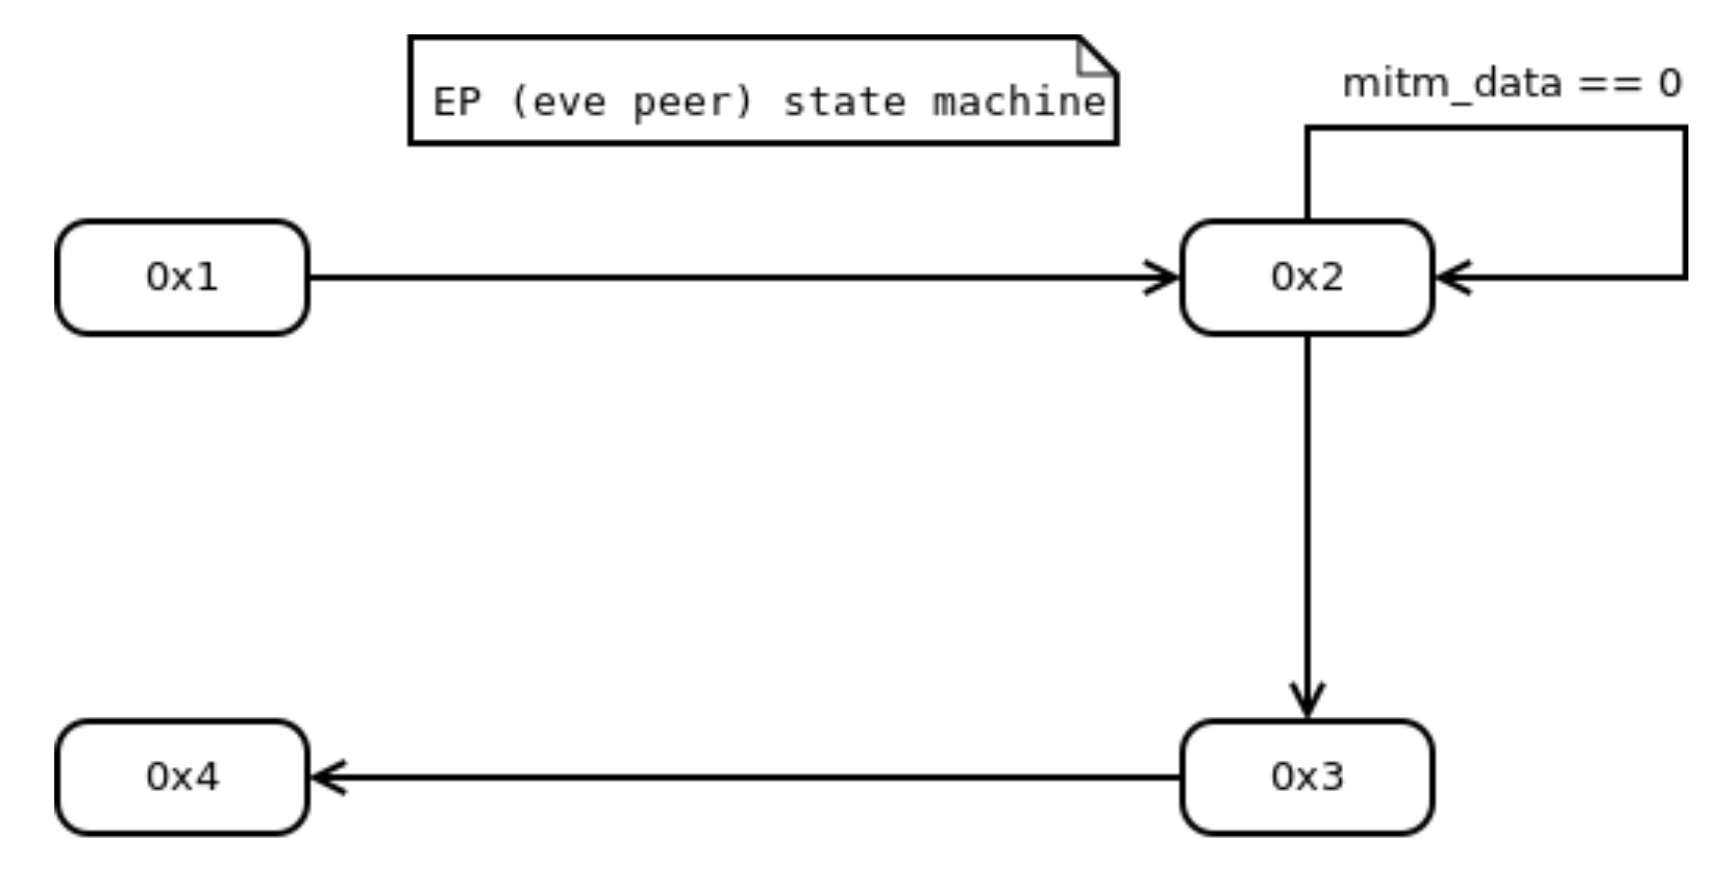
\includegraphics[scale=0.5]{res/eve-peer-mitm-state-machine-diagram.png}

  0x1 $\rightarrow$ 0x2
  \begin{enumerate}
    \item Посылка сообщения протокола MITM с MSCHAPv2 Challenge
      Request от AS(Сервера Алисы)
  \end{enumerate}

  0x2 $\rightarrow$ 0x3
  \begin{enumerate}
    \item Получение сообщения протокола MITM с MSCHAPv2 Challenge
      Response от BP (Клиента Боба)
    \item Конструирование поддельного MSCHAPv2 Challenge
      Response используя приобретённый Challenge Response
  \end{enumerate}

  0x3 $\rightarrow$ 0x4
  \begin{enumerate}
    \item Посылка сообщения протокола MITM с MSCHAPv2 Challenge
      Response от BP(Клиента Боба)
    \item Конструирование поддельного MSCHAPv2 Success
      Response без проверки Authenticator Response в Success Request
  \end{enumerate}
  \caption{Автомат Клиента MitM}
\end{figure}

\begin{figure}
  \centering 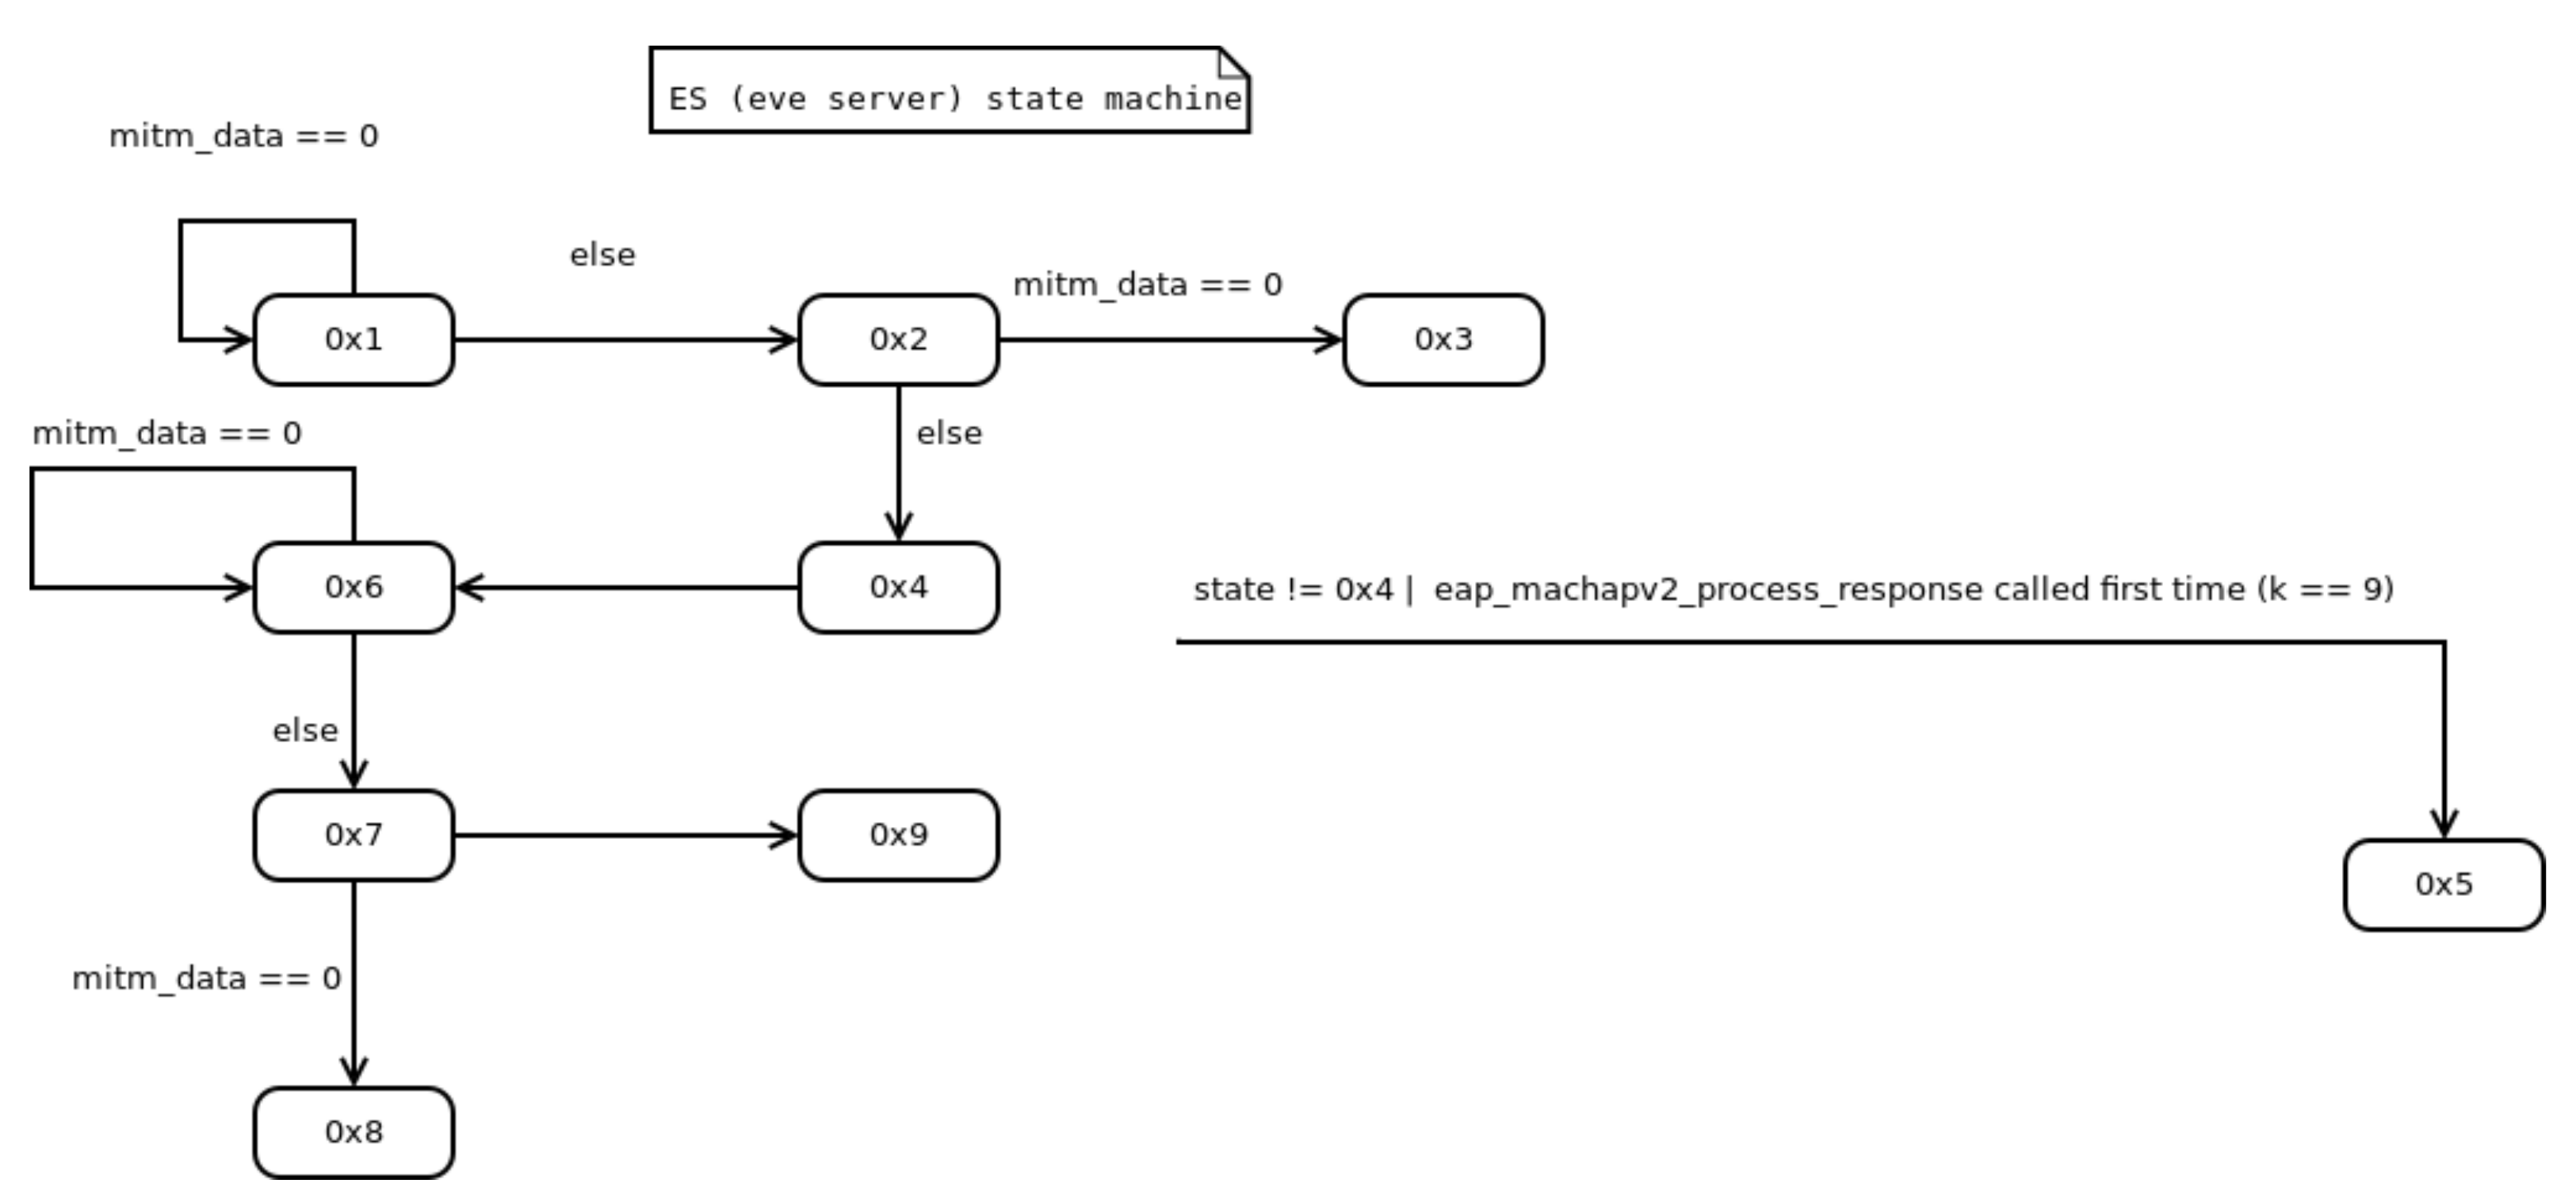
\includegraphics[scale=0.5]
    {res/eve-server-mitm-state-machine-diagram.png}
  0x1 $\rightarrow$ 0x2
  \begin{enumerate}
    \item Recieve MITM protocol message: MSCHAPv2 Challenge
      Request from AS (alice server)
  \end{enumerate}
  0x2 $\rightarrow$ 0x3, 0x* $\rightarrow$ 0x5, 0x7 $\rightarrow$ 0x8
  \begin{enumerate}
    \item Failure
  \end{enumerate}
  0x2 $\rightarrow$ 0x4
  \begin{enumerate}
    \item Build Forged MSCHAPv2 Challenge
      Request using obtained auth\_challenge and server\_id
  \end{enumerate}
  0x4 $\rightarrow$ 0x6
  \begin{enumerate}
    \item Transmit MITM protocol message with MSCHAPv2 Response from BP(bob peer)
  \end{enumerate}
  0x6 $\rightarrow$ 0x7
  \begin{enumerate}
    \item Receive MITM protocol message MSCHAPv2 Success
      Request from AS (alice server)
    \item Skip Challenge Response verification,
      state = SUCCESS\_REQ, master\_key\_valid=1
  \end{enumerate}
  0x7 $\rightarrow$ 0x9
  \begin{enumerate}
    \item Build Forged MSCHAPv2 Success Request using obtained success request
  \end{enumerate}
  \caption{Автомат Сервера MitM}
\end{figure}

The eap\_example code triggers state machines to make a step one by one,
and if there is some new message produced, the loop iteration repeats.
In a real life, all of the state machines will operate in parallel,
and on different devices.
The physical communication is the task of EAPOL state machine,
i.e. EAP over LAN.
It is responsible for operation of EAP state machine and the delivery
of its messages.
The communication between pairs of Bob Peer and Eve Server,
and Eve Peer and Alice Server state machines occurs naturally
as Eve Peer likely to be wpa\_supplicant instance, and Eve Server is to be the
instance of hostapd.
The rest two machines, are of no concern to the attacker.
To connect MitM state machines, we are likely to use socket communication.
But I repeat again, that we present only simulation.
And here all packets are transmitted via simple buffer copying within one process.

\section{Development summary}

Here is presented a summary of how simulation behaves
with every commit applied on top of the previous one.

\textbf{commit 242fc738a057}

Peer is authenticated by Server within a TLS 1.2 tunnel,
with a help of PEAPv0 with MSCHAPv2. By the end of conversation
TLV Cryptobinding protocol is performed.

\textbf{commit 3d38acc54e62}

EAP behaviour is the same. Commits contains not related changes.

\textbf{commit cf8b14eb9c93}

EAP behaviour is the same. But secret material is revealed in log,
i.e. TLS master secret, EAP keying material and etc.

\textbf{commit 26d71ce309d3}

EAP behaviour is the same. EAP state machine data was incapsulated
into instance\_data structure. See commit message for more details.

\textbf{commit c08e56344833}

The EAP behaviour was duplicated. Two pairs of state machines
communicate between each other - Bob Peer and Eve Server,
and Eve Peer and Alice Server.

\textbf{commit 024a2b3685aa}

Bob Peer was configured to skip network certificate verification
obtained from Eve Server.

\textbf{commit 9a2cd78574c6}

Bob Peer forces PEAPv1, the same actions are taken
by Alice and Eve Server. It alleviates TLV Cryptobinding
as well as forces EAP keying material to be derived
from TLS master secret only.

\textbf{commit bc0150b8dadb}

Eve Peer and Eve Server are delayed for some time.
To achieve the behaviour pending request and pending response
functionality of hostap implementation was utilized.

Both Eve Peer and Eve Server are waiting 10 iterations
processing the very same packets -- MSCHAPv2 Challenge Request
for Eve Peer,
and EAP-Identity Response for Eve Server.
After 10 iterations they proceed with usual behaviour.

\textbf{commit b88c9c348287}

Eve Peer puts MSCHAPv2 Challenge and server\_id into mitm\_data
buffer and remains in pending state as usual.
Eve Server waits for a new message,
after that he continues usual behaviour of EAP-Identity Phase2 method.

So despite of the message transmission,
Eve's state machines end up as usual after waiting iterations.

Both pairs still communicates independently as in default eap\_example.

\textbf{commit 7964f349cbbe}

Eve Server generate MSCHAPv2 Challenge Request with a challenge
from Alice Server.

The communication ends up succefully, as Eve Server possesses
user identity and password.

There is no simulation, except for generating random challenge
by Alice Server only. And Eve Server takes it, by receiving
a message from Eve Peer MitM state machine, to generate
challenge request.

\textbf{commit  764f22d88a12}

EAP behaviour is the same. Commit enables CONFIG\_TESTING\_OPTIONS
to generate asleap utility commands. Such a behaviour
resembles the attack from SHMOOCON presentation.

In other words, we can start up a hostapd instance, which
has the name of a target NAS. And to repeat the attack
all we need is to enable asleap commands generation.

By the end of communication log will contain proper
dictionary attack commands for all clients, that
were trying to authenticate at our server.

\textbf{commit 0ccda46808674}

Eve Server MitM state machine transmits MSCHAPv2 Challenge
Response obtained from Bob Peer to Eve Peer MitM state machine.
Eve Server ignores
all response verification routins as well as MSCHAPv2 master
key derivation. It will be user later, when replying with a forged
MSCHAPv2 Success Request.

The simulation is still not correct,
as by the end of  waiting loop, Eve Server takes user password
to verify Challenge Response and generate Success Request.

Eve Peer also authenticates correctly, because the only alteration
is transmission of Challenge Request from Alice Server to Eve Server.
Eve Peer as well uses the same password as Bob Peer.

\textbf{commit 1a1149e963aca}

Eve Peer sends to Alice Server correct challenge response,
botained by Eve Peer MitM state machien from Eve Server MitM state machine.
Alice Server authenticates Eve Peer.
But Eve Peer fails to accept success requst from Alice Server
as the default eap\_example behaviour should do.
Because MSCHAPv2 Peer Challenge is not equal to the one produced by Bob Peer.
In further commits, Eve Peer will simply ignore this verification
as the protocol relies on user consciousness only.
And it is right, since Eve Peer is the attacker,
and the legitimate client.

For now we may say that the simulation is partially succeeded.
Since the attacker was authenticated by original server,
and all we need is to properly finish MSCHAPv2 Sucess Request verification
and reply with a proper MSCHAPv2 Success Response, that doesn't
require any special knowledge from Eve Peer.

The only reason to forge MSCHAPv2 Success Request for Bob Peer
is to make him tunneling his network traffic through MitM node.

\textbf{commit 4a46fa992e7ca}

Eve Peer catches Success Request from Alice Server.
Eve Peer MitM state machine transmits the message to Eve Server MitM state machine,
which receives the message and resume Eve Server Eap state machine operation.

The next step by Eve Server is to built a forged MSCHAPv2 Success Request,
with a help of the one generated by Alice Server and obtained by Eve Peer.

To the moment, both Eve Peer and Bob Peer marks MSCHAPv2 Success Request
as invalid. The one doesn't posses correct secret material,
whereas another one, Bob Peer, receives an incorrect request.

\textbf{commit 9cebe623049fe}

Eve Server applies obtained MSCHAPv2 Success Request to generate
a proper Request for Bob Peer. That the one happily accepts.
The conversation between Eve Server and Bob Peer finishes successfully.
Both parties derive the same keying material based solely on TLS master secret.
From this moment Bob Peer should begin
its network activity, encrypted by keying material known to Eve Server.

To finish the attack simulation, we need to authenticate Eve Peer,
because the network resource is in possession of Alice Server.

\textbf{commit 45d1094c7494c}

Клиент Евы игнорирует проверку MSCHAPv2 Success Request
и отвечает с MSCHAPv2 Success Response.
Общение между Клиентом Евы и Сервером Алисы
завершается успешно. Обе стороны производят
один и тот же материал для создание ключей
основанный только на главенствующем секрете TLS.
С этого момента Сервер Алисы должен принимать
сетевой траффик, и данные будут шифроваться с помощью
ключа известного Клиенту Евы.

В реальной атаке человек-по-середине, Сервер Евы
и Клиент Евы должны начать проброс сообщений между Клиентом Боба
и Сервером Алисы.
Они оснащены всеми необходимыми ключами для компрометирования
туннелей.
Как преимущество атаки,
Ева может слать любые дополнительные сетевые сообщения,
поскольку имеется полностью аутентифицированный и авторизованный
доступ к сети.
В атаке человек-по-середине, главная цель это анализ траффика жертвы.
Данная цель достигнута успешно.

\section{Заключение}
Я бы хотел сказать, что симуляция была успешной
и благодяра хорошей кодовой базе hostap,
не отняла много времени при реализации.
Хотя мы можем только мечтать о её применении в реальной жизни.

\begin{thebibliography}{99}
  \bibitem{tap2002}
    Man-in-the-Middle in Tunneled Authentication Protocols \\
    http://eprint.iacr.org/2002/163/
  \bibitem{GMI}
    https://github.com/nartes/hostap-mitm-mschapv2-peapv1
  \bibitem{josefsson-draft-05}
    https://tools.ietf.org/html/draft-josefsson-pppext-eap-tls-eap-05
  \bibitem{josefsson-draft-10}
    https://tools.ietf.org/html/draft-josefsson-pppext-eap-tls-eap-10
  \bibitem{rfc4137}
    https://tools.ietf.org/pdf/rfc4137.pdf
  \bibitem{hostap-w1fi}
    http://w1.fi/
  \bibitem{hostapd-wpe}
    https://github.com/OpenSecurityResearch/hostapd-wpe
  \bibitem{whfs-peap-shmoocon-2008}
    http://www.willhackforsushi.com/presentations/\\
    PEAP\_Shmoocon2008\_Wright\_Antoniewicz.pdf
\end{thebibliography}
\end{document}
